\documentclass[20pt]{article}
\usepackage{graphicx}
\usepackage{float}


\title{EECS 112L Lab2 Report}
\author{Jay Patel\\ \vspace{0.5cm} ID: 77742251\\ Professor Pooria M. Yaghini}

\begin{document}
\maketitle
\pagenumbering{arabic}
\newpage
\section{Block Diagram of the design Implementation}

In this Section, I aim to describe my design of a single cycle processor.In addition, I present a brief description on how each Instruction type is implemented and supported by the processor. \\\\
The original processor only allowed execution of R-type and I-type(Load,ADDI) instructions.

\begin{figure}[H]
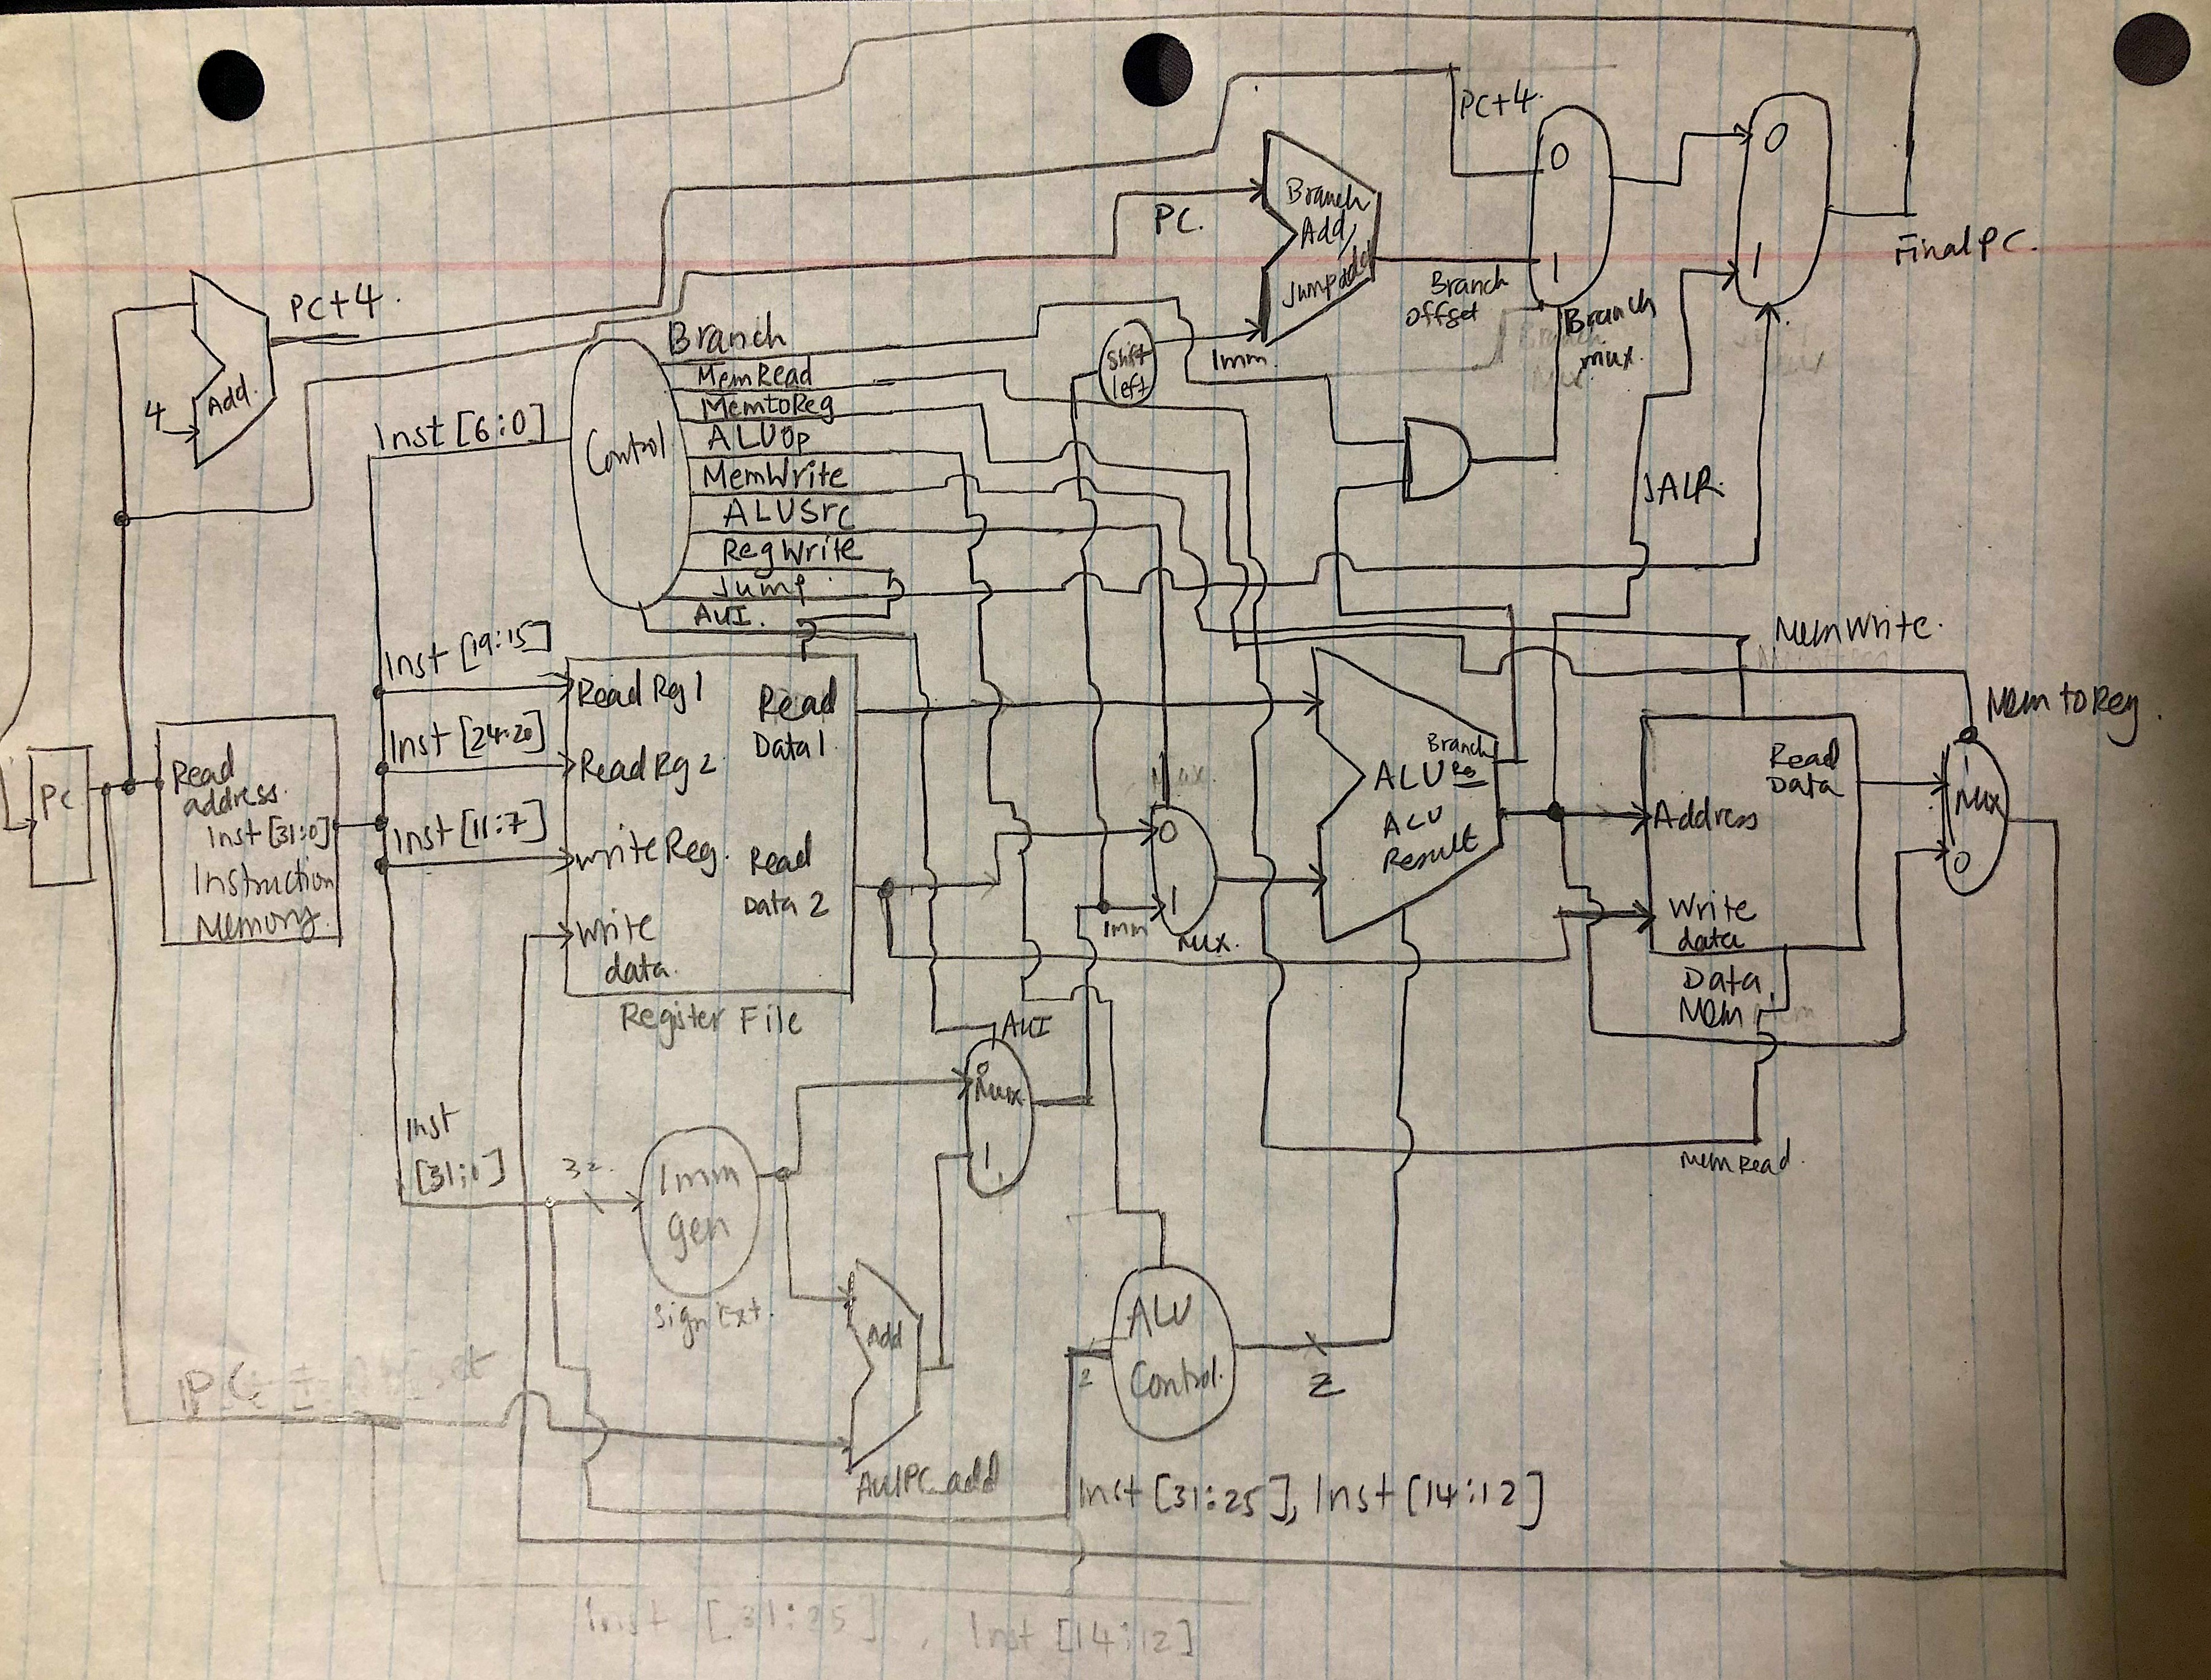
\includegraphics[width=\linewidth,height=7cm]{design.jpg}
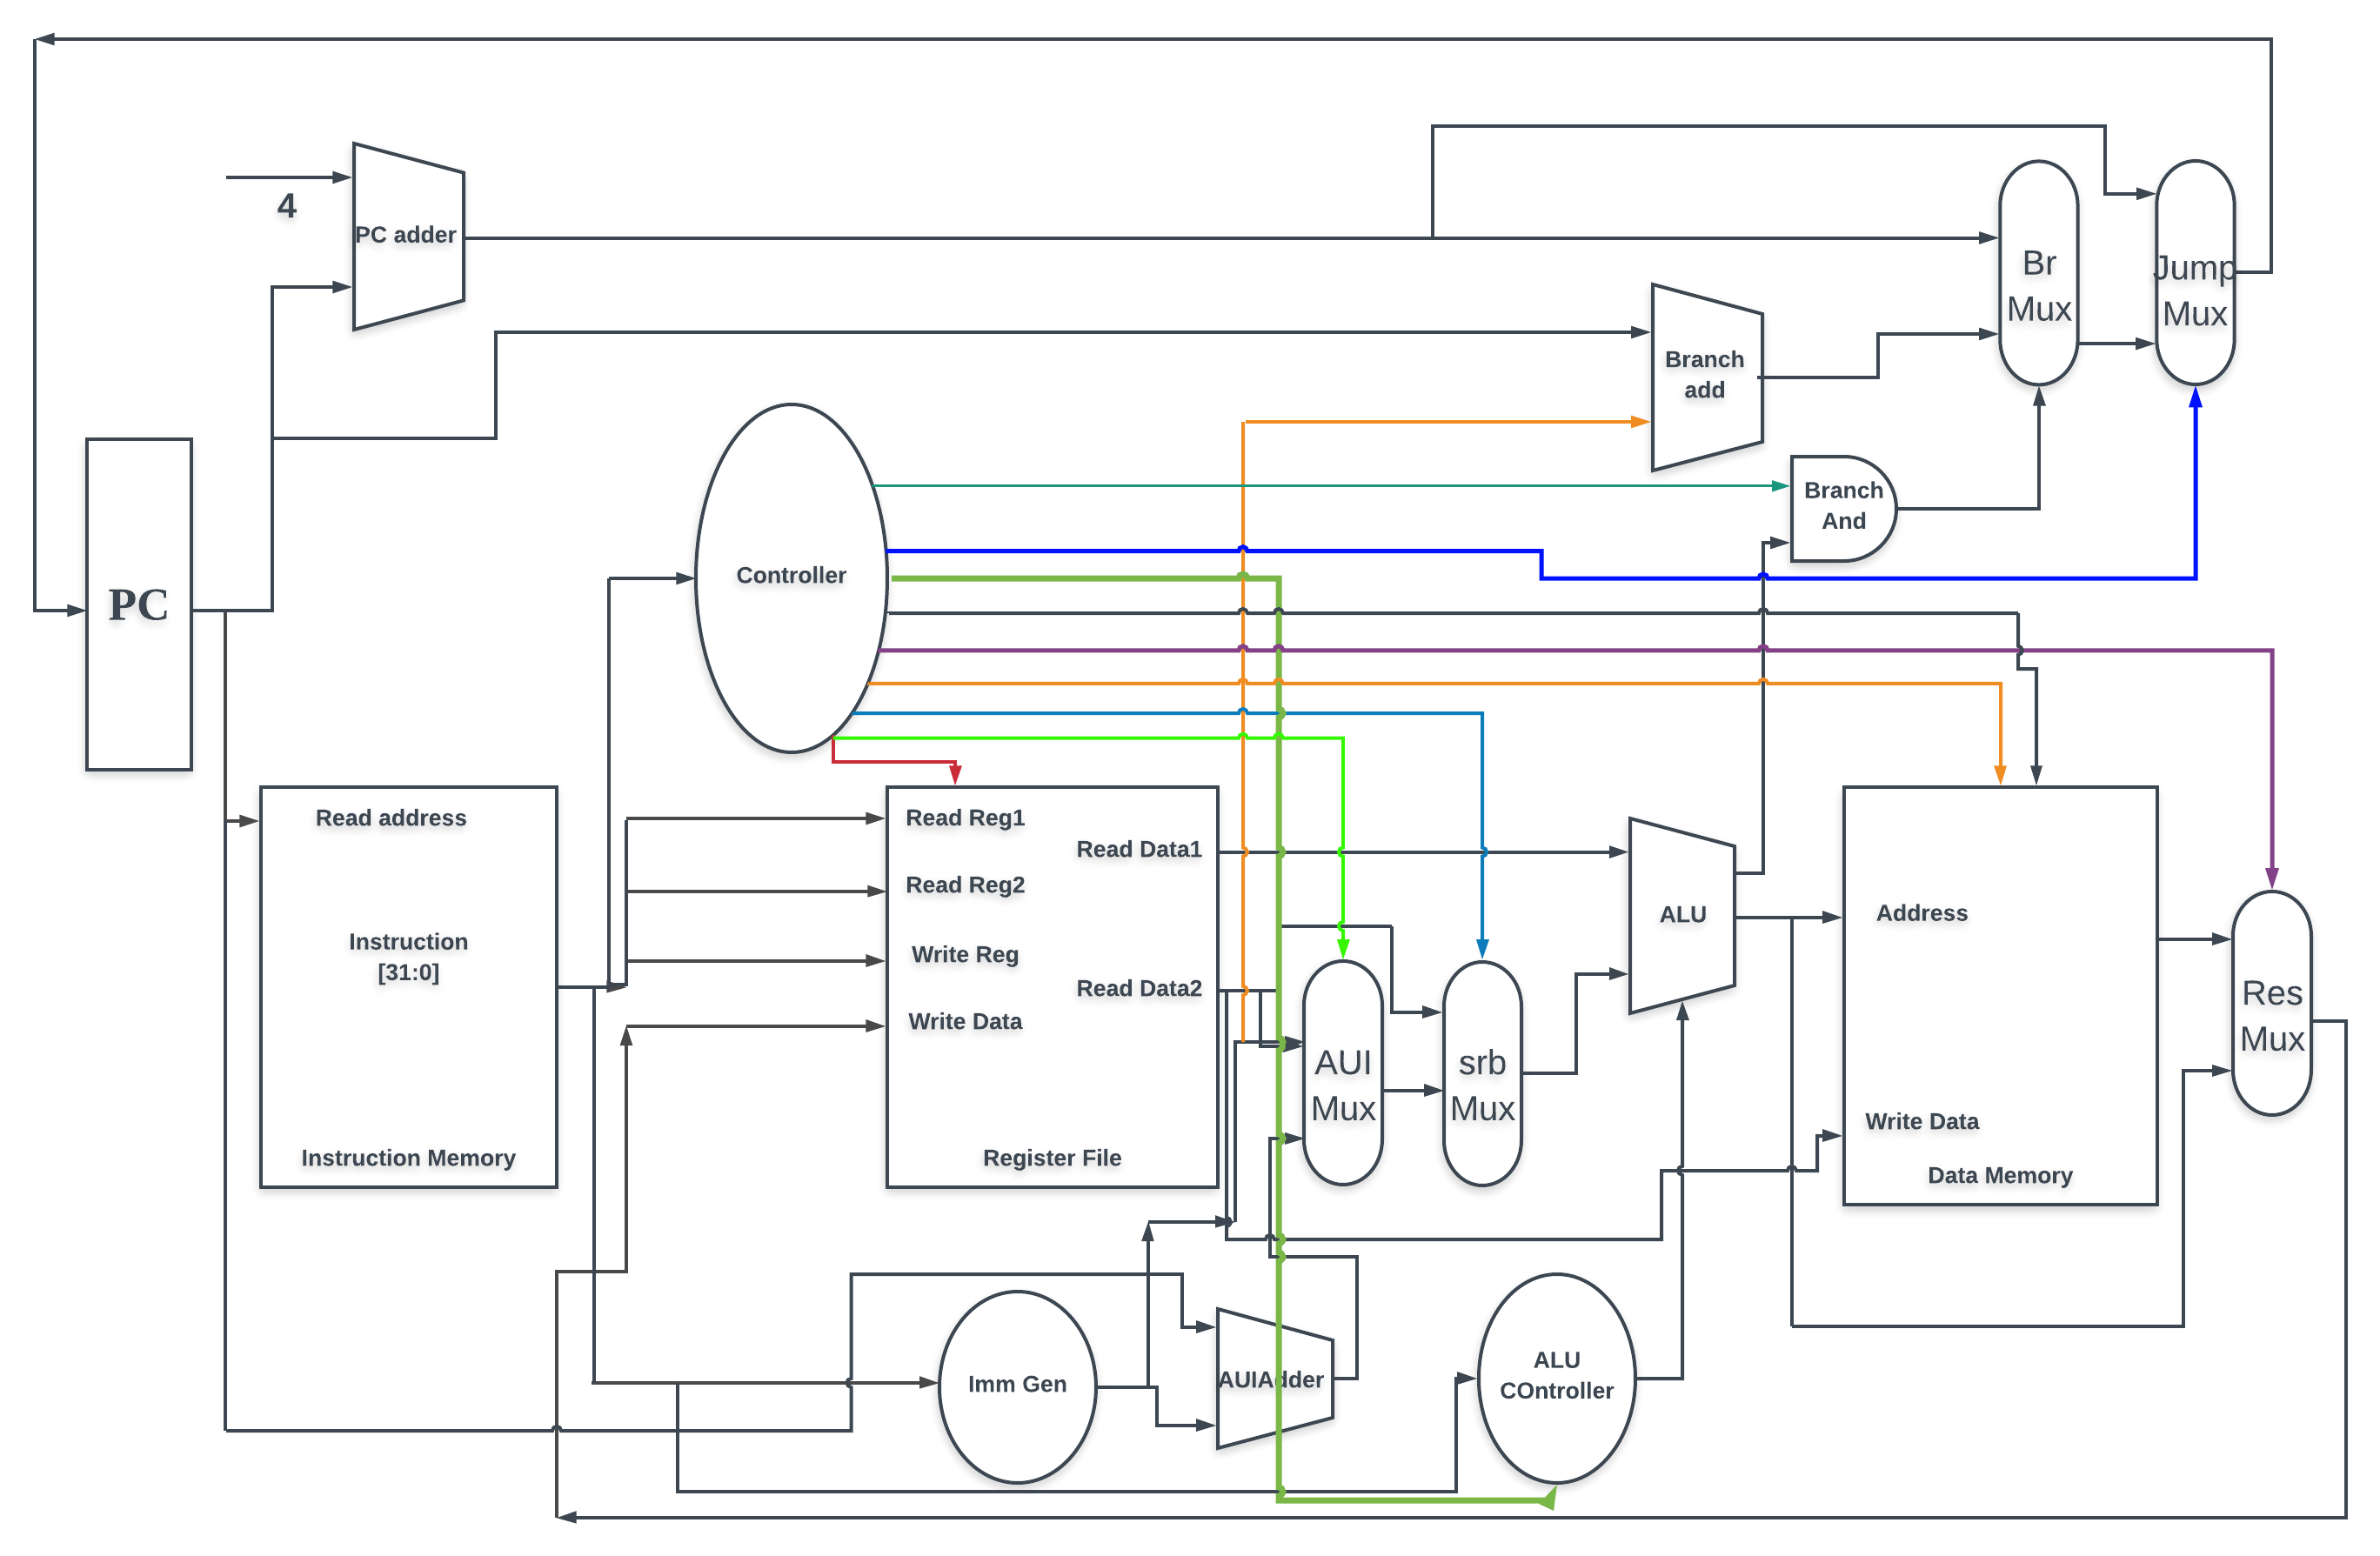
\includegraphics[width=\linewidth,height=7cm]{Datapath}
\caption{Complete Design of Single Cycle processor}
\end{figure}
In addition to the original instructions supported in Lab 1, this processor is aimed to execute the following instruction types:

\begin{itemize}
    \item Integer Register-Register Instructions(R-type)
    \item Integer Register-Immediate Instructions(RI-type)
    \item Load Instructions
    \item Store Instructions
    \item Conditional Branch Instructions
    \item Jump( JAL, JALR) Instructions
    \item Load Upper Immediate(LUI), Add Upper Immediate to PC(AUIPC)
\end{itemize}
\newpage
\subsection{Integer Register-Register Instructions(R-type)}

\begin{figure}[H]
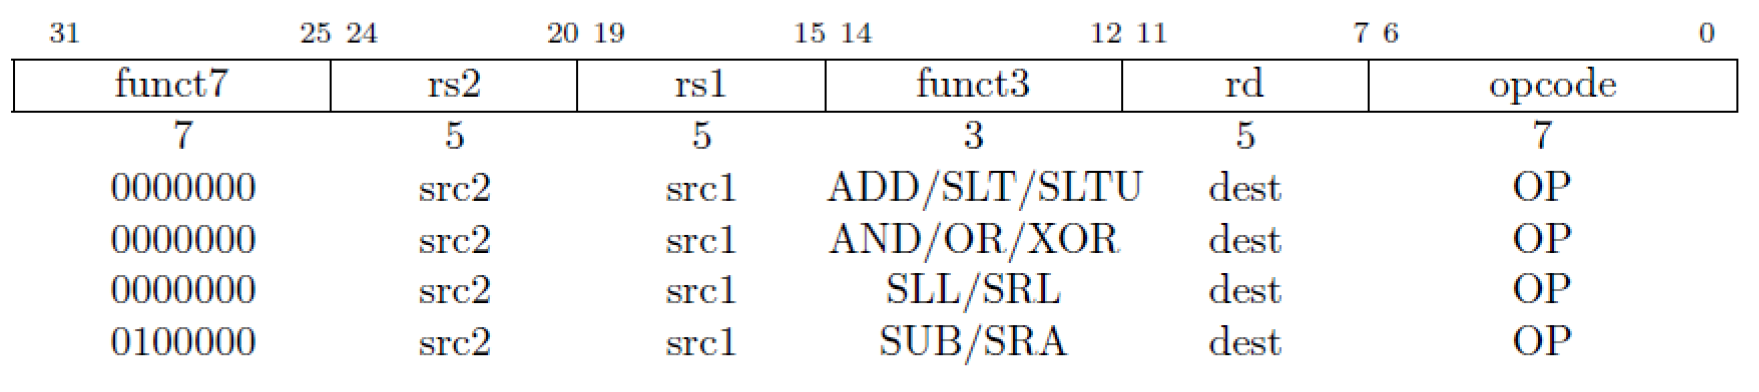
\includegraphics[width=\linewidth]{RType}
\caption{Snippet of R-type instructions}
\end{figure}

For R-type, the register file module provides the two register source operands.The first operand, RS1 is wired directly to Input 1 of ALU.RS2 is connected to a 2-1 multiplexer. The control signal ALUsrc will be 0 for this mux to pass RS2 operand as the output for Input 2 of ALU. Meanwhile, using funct3 operand (Inst[14:12]) and funct7 operand (Inst[31:25]),ALUcontroller will set ALU operation bits according to various instructions like ADD, AND, OR, SLL, etc. Then the ALU will execute the instruction based on operation and turn on necessary flags to send the result to the destination register.

\begin{figure}[h]
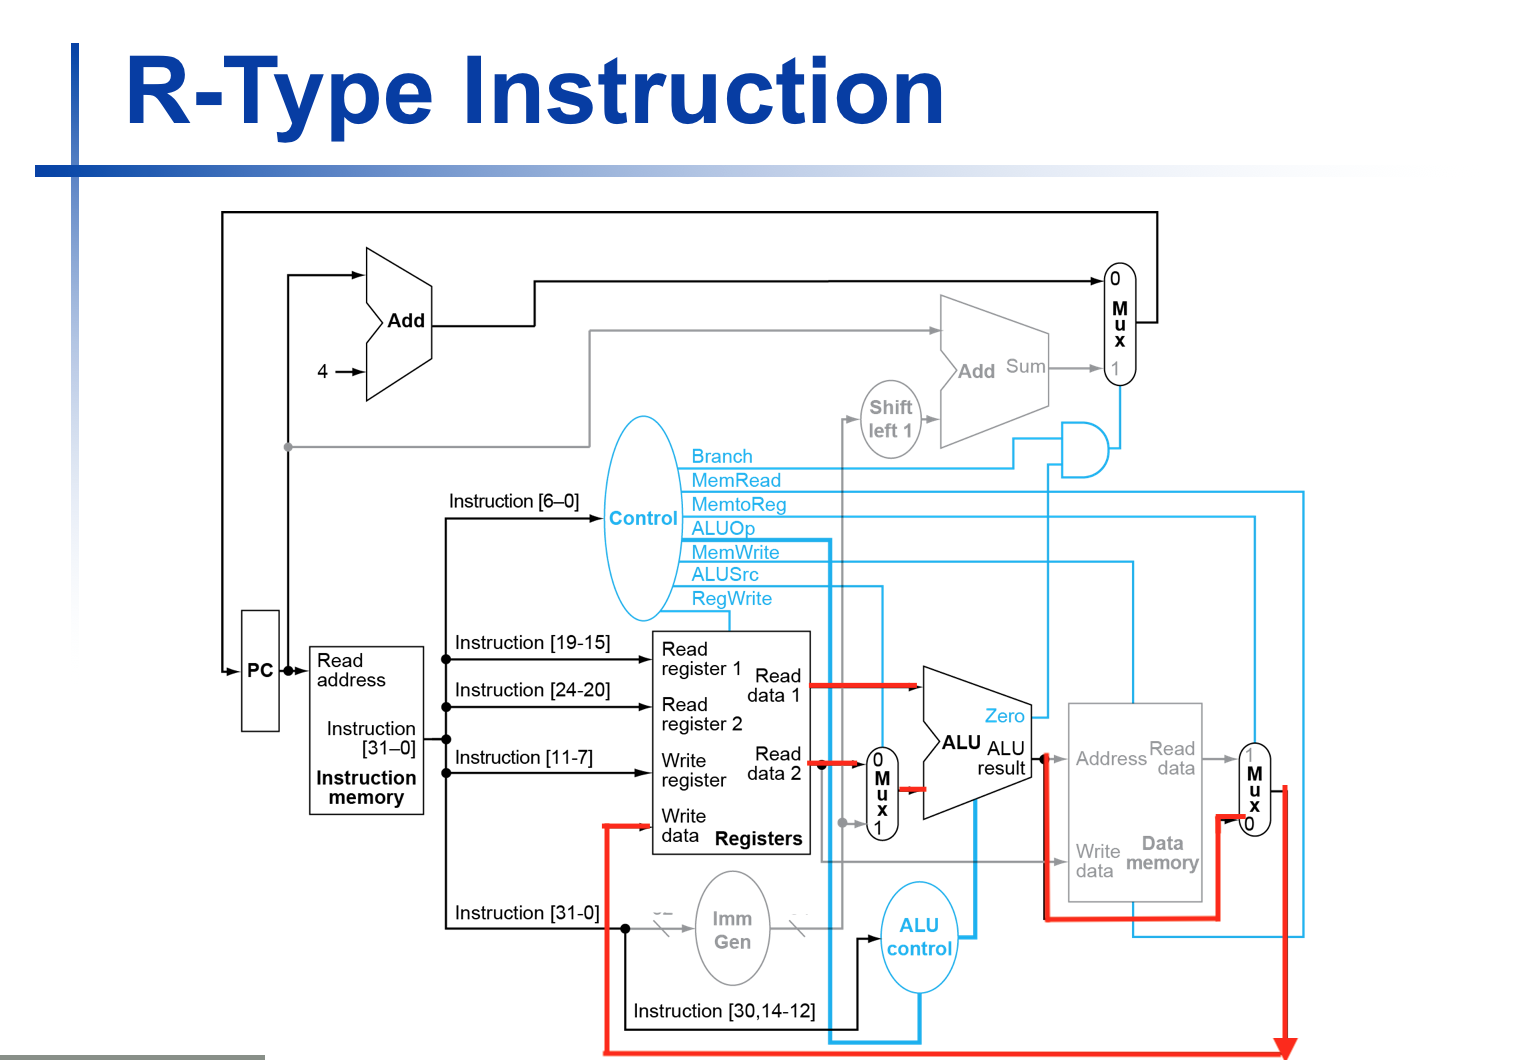
\includegraphics[width=\linewidth]{Rtypepath}
\caption{R-type datapath}
\end{figure}

\subsection{Integer Register-Immediate Instructions(RI-type)}

\begin{figure}[h]
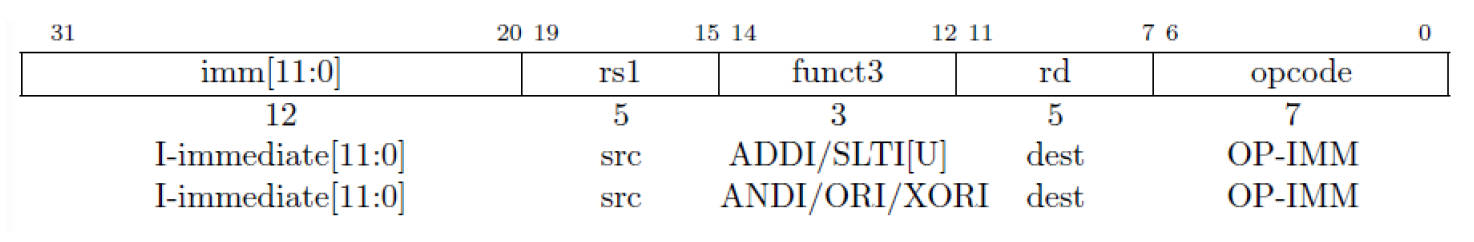
\includegraphics[width=\linewidth]{RI-type}
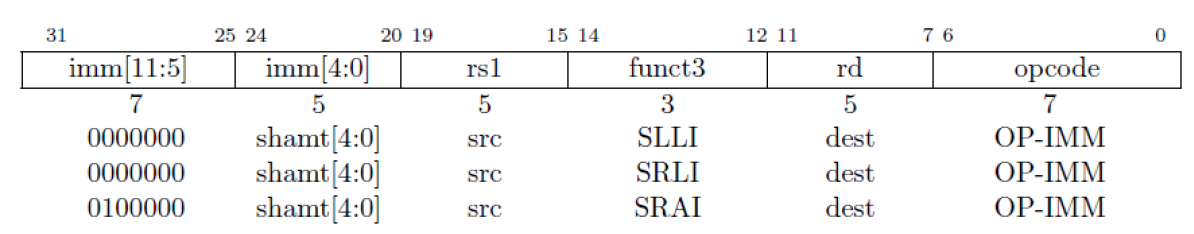
\includegraphics[width=\linewidth]{SI-type}
\caption{Snippet of RI-type instructions}
\end{figure}

For RI-type, the register file module provides the a register source operand and an immediate field of 12 bits.The first operand, RS1 is wired directly to Input 1 of ALU. The immediate value is connected to a module called ImmGen, where the immediate value is sign extended to 32 bit value. The output of ImmGen is connected to a 2-1 multiplexer. The control signal ALUsrc will be 1 for this mux to pass the immediate value as the second source operand for Input 2 of ALU. Meanwhile, using funct3 operand (Inst[14:12]) and funct7 operand (Inst[31:25]),ALUcontroller will set ALU operation bits according to various instructions like ADDI, ANDI, SLLI, etc. Then the ALU will execute the instruction based on operation and turn on necessary flags to send the result to the destination register.

\begin{figure}[h]
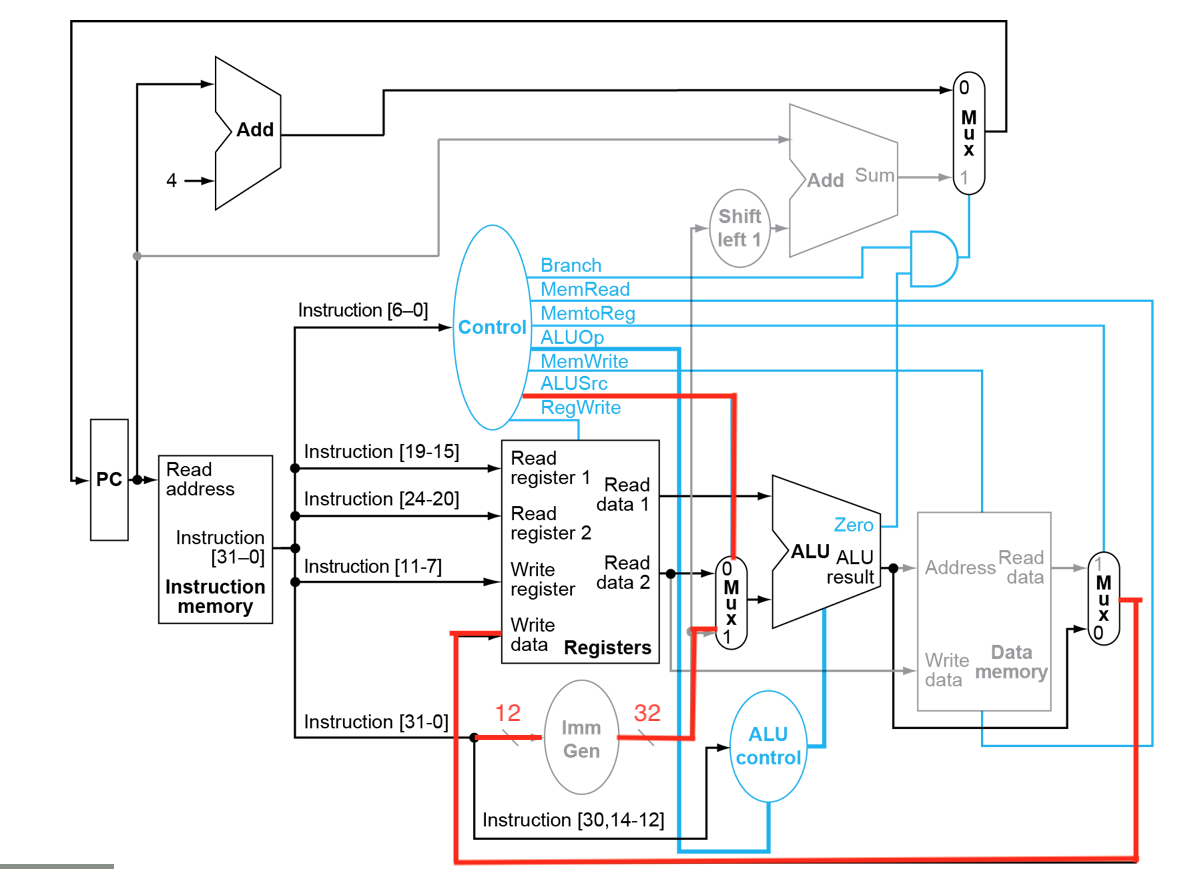
\includegraphics[width=0.9\linewidth, height=6cm]{RIdatapath}
\caption{Snippet of RI-type instruction datapath}
\end{figure}

\subsection{Load Instructions}

\begin{figure}[h]
	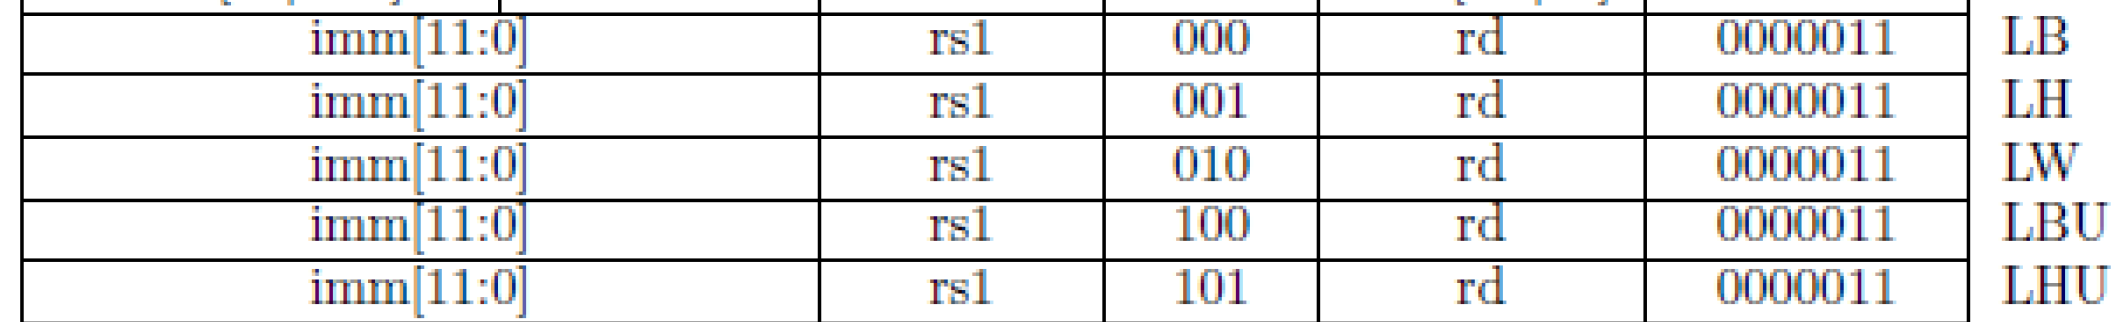
\includegraphics[width=\linewidth]{Load}
	\caption{Snippet of Load instructions}
\end{figure}

For Load, the immediate gen module will sign extend the immediate value and then a mux will select, based on the ALUSrc flag,  second source operand as the immediate.Then the ALU will execute the instruction by adding immediate value to source operand 1. The Alu result is an address for the data memory, where the value at the address corresponding to load-type(LB, LH, LW, LBU,or, LHU) is written into the destination register. 

\begin{figure}[H]
	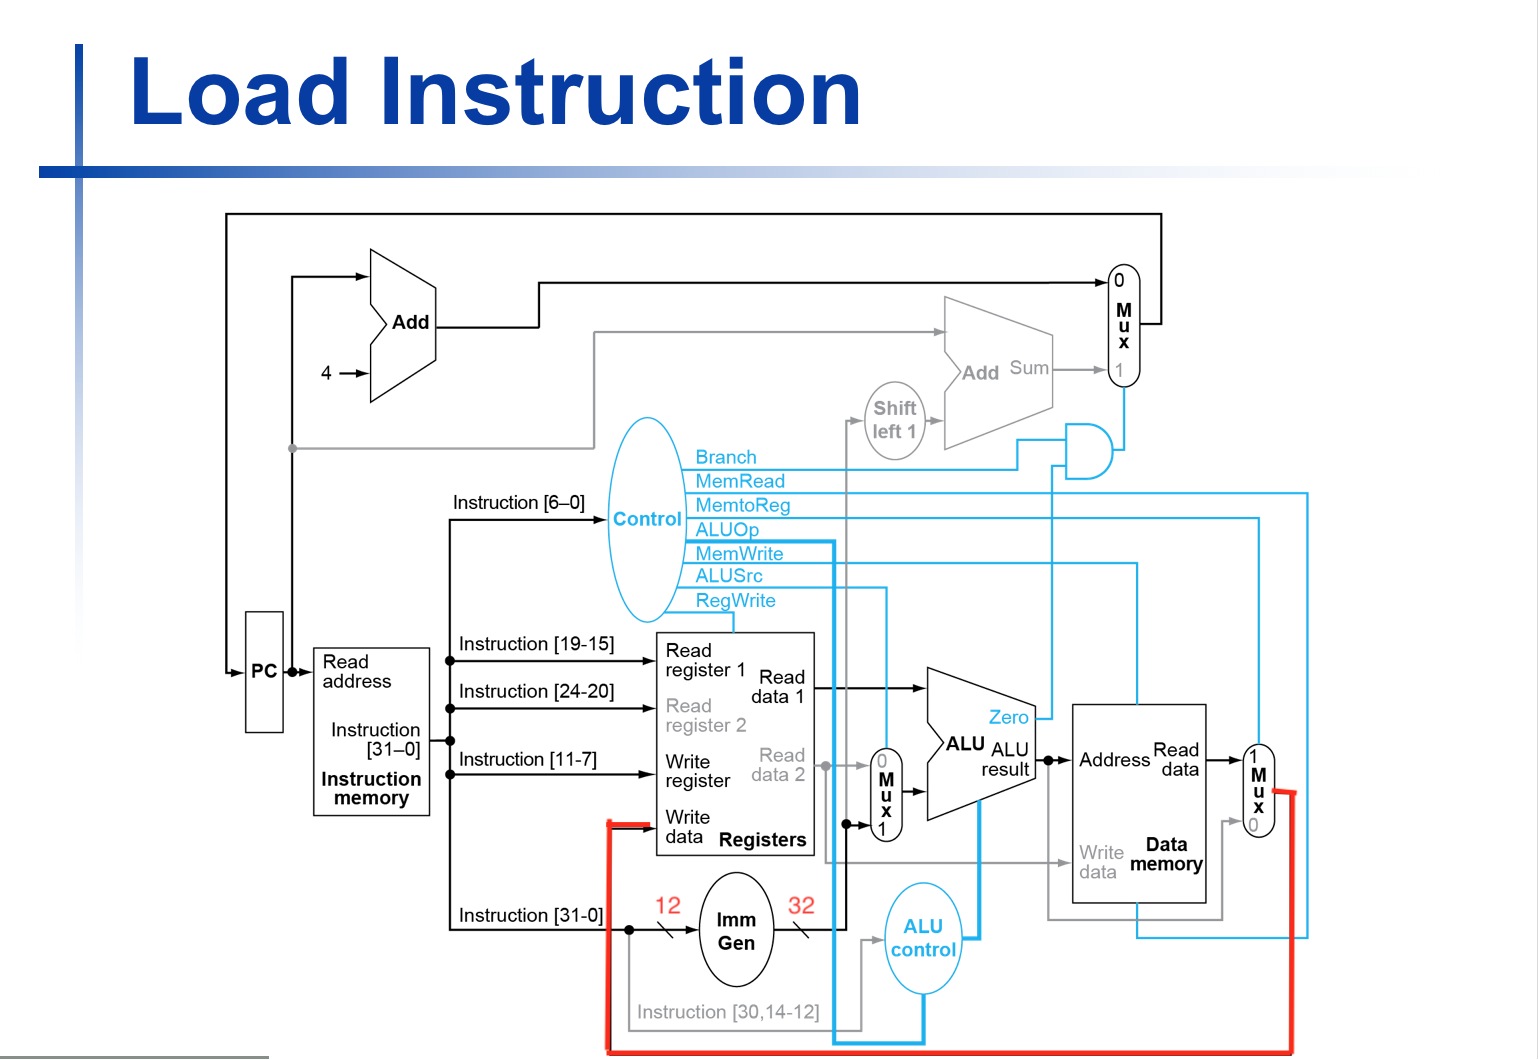
\includegraphics[width=\linewidth,height=10cm]{LoadDatapath}
	\caption{Load Datapath}
\end{figure}

\subsection{Store Instructions}
\begin{figure}[H]
	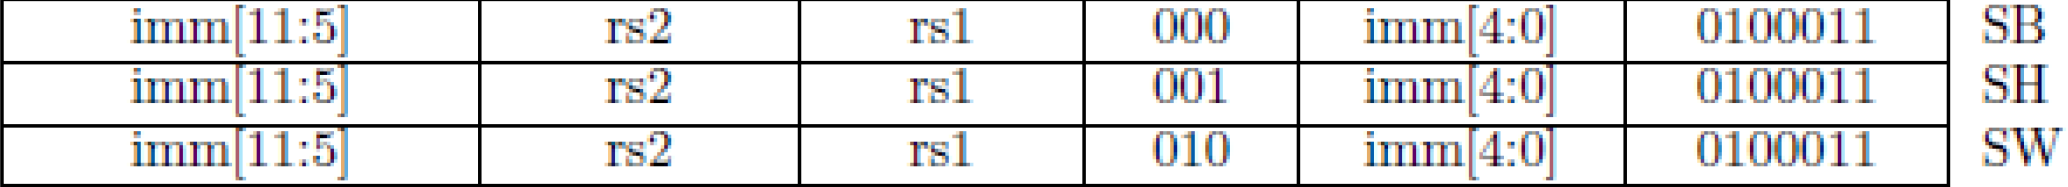
\includegraphics[width=\linewidth]{Store}
	\caption{Snippet of Store instructions}
\end{figure}

For store, the immediate gen module will sign extend the immediate value and then a mux will select, based on the ALUSrc flag,  second source operand as the immediate.Then the ALU will execute the instruction by adding immediate value to source operand 1. The Alu result is an address for the data memory, where the value at the address in the data memory  will be overwritten with  values corresponding to store-type(SB, SH, SW). 

\begin{figure}[H]
	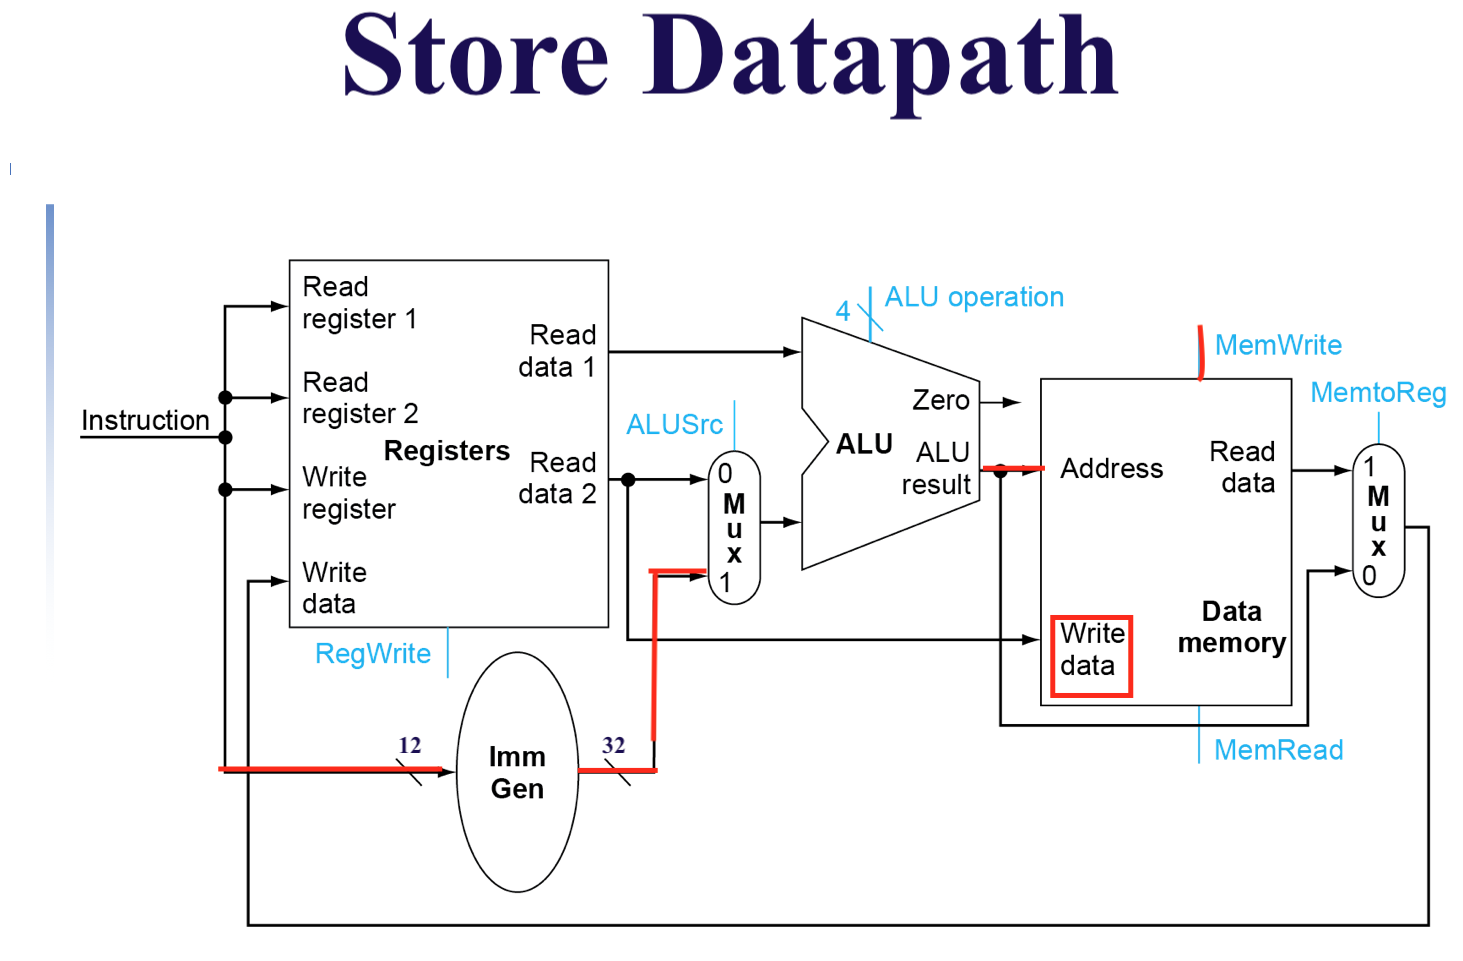
\includegraphics[width=\linewidth]{Storedatapath}
	\caption{Store instructions Datapath}
\end{figure}

\newpage
\subsection{Conditional Branch Instructions}

\begin{figure}[H]
	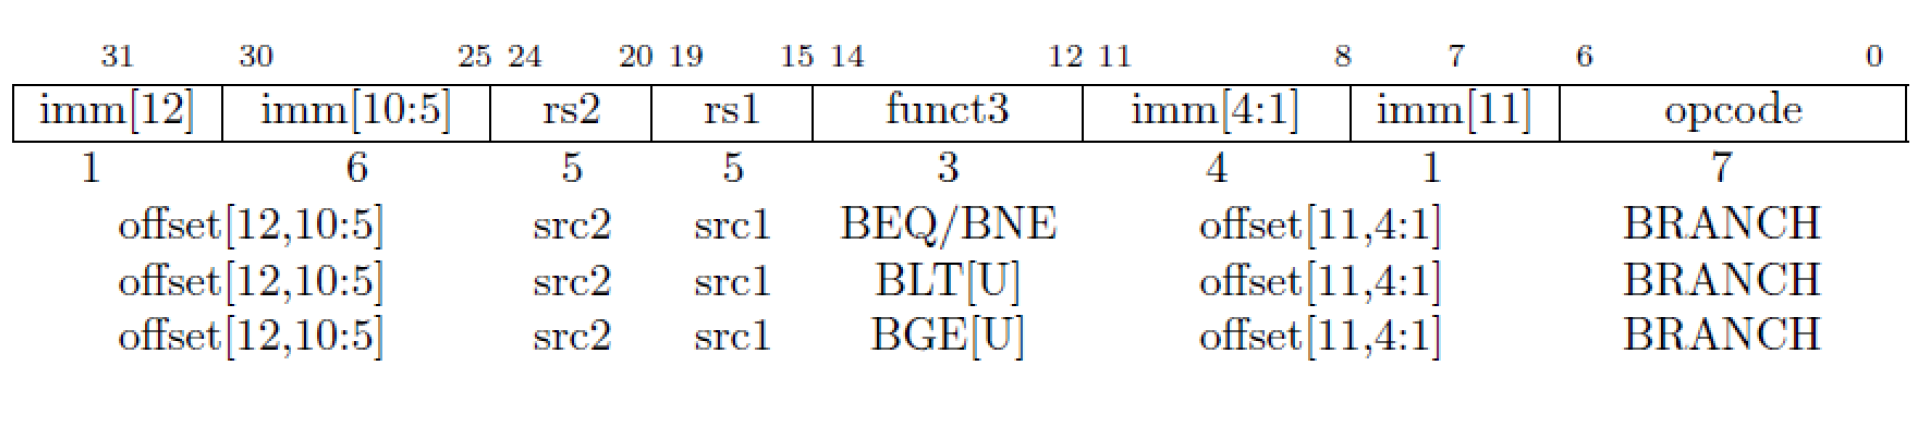
\includegraphics[width=\linewidth]{Branch}
	\caption{Snippet of Branch instructions}
\end{figure}
For branch, the immediate gen module will sign extend the immediate and then a mux will select, based on the ALUSrc flag, second source operand as the immediate. Then the ALU will execute the instruction based on operation using Function 3 of the instruction. and turn on necessary flags to send the result a branch andgate, which will set the branch signal to 1 if both the branch control signal and the signal based on ALU result. If the branch signal is 1, the new Pc will be the branch offset + PC and if branch signal is 0, then the New Pc will be PC+ 4. 

\begin{figure}[H]
	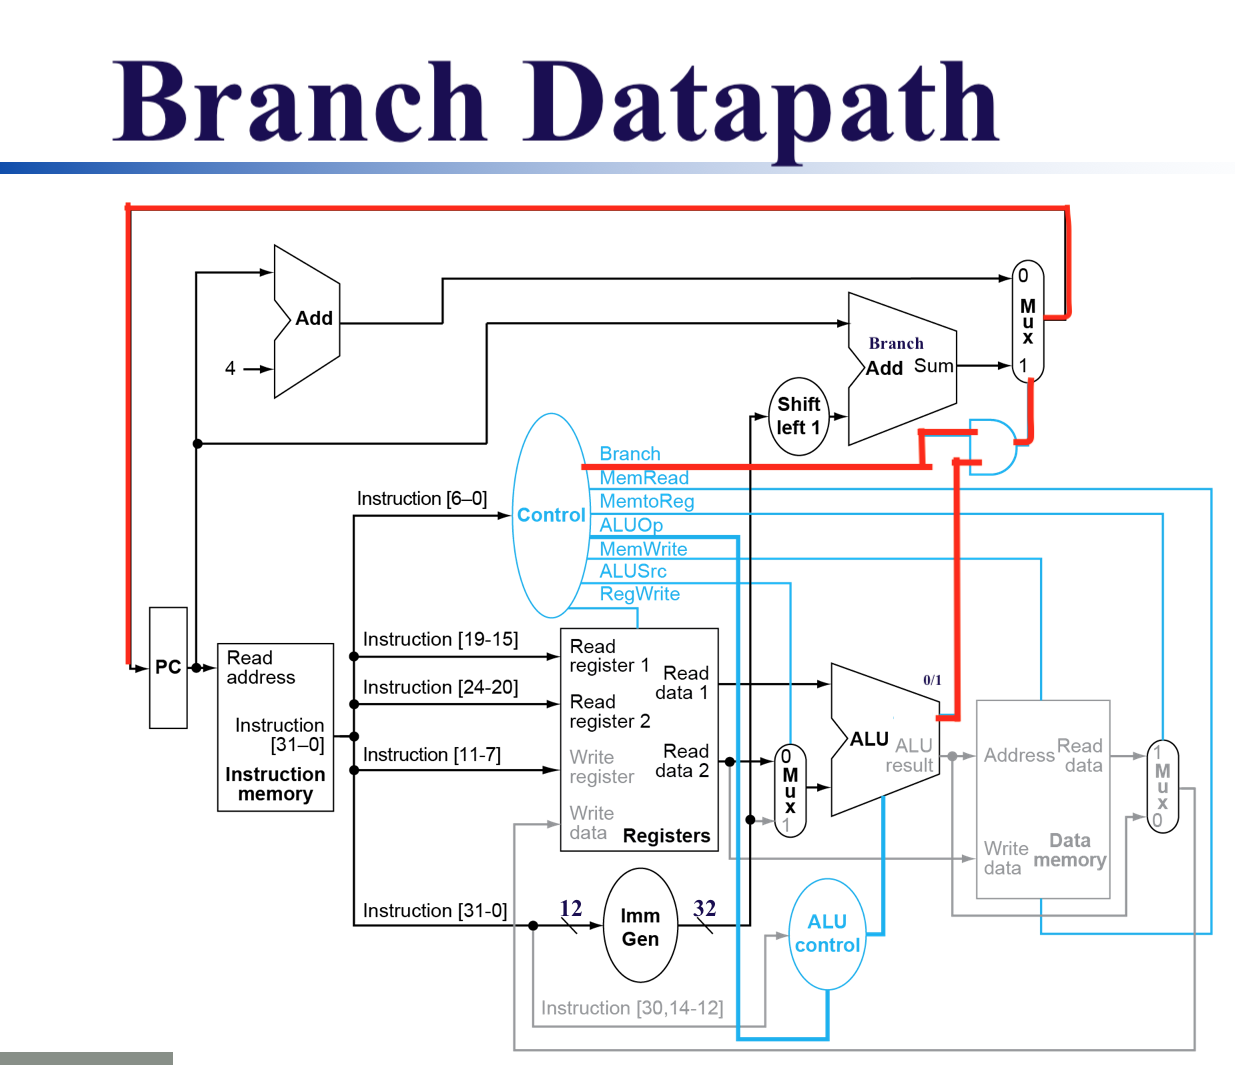
\includegraphics[width=0.9\linewidth]{Branchdatapath}
	\caption{Branch instructions Datapath}
\end{figure}

 \subsection{Load Upper Immediate(LUI), Add Upper Immediate to PC(AUIPC)}

\begin{figure}[H]
	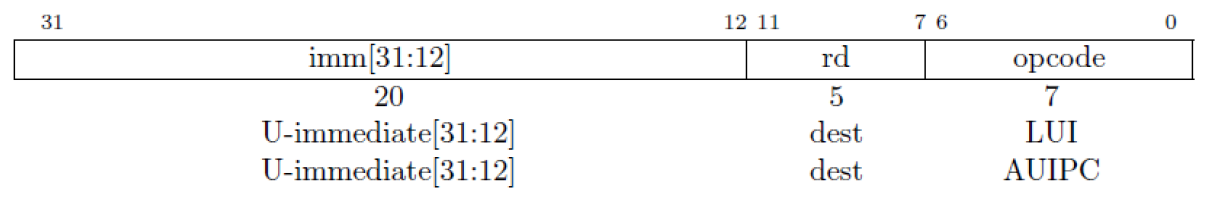
\includegraphics[width=\linewidth]{Utype}
	\caption{LUI/AUIPC instructions }
\end{figure}

For LUI, the immediate gen module will sign extend the immediate and then a mux will select the immediate value, based on the ALUSrc flag .Then, the ALU will execute the instruction based on operation for LUI, and so the upper 20 bits of the immediate value will be written back to the destination register.

For AUIPC, the immediate gen module will sign extend the immediate and then a mux will select the immediate value, based on the ALUSrc flag. Then, the immediate value will be added to the PC to get the new value. Then, the ALU will execute the instruction based on operation for AUIPC, and so the upper 20 bits of the value will be written back to the destination register.

\begin{figure}[H]
	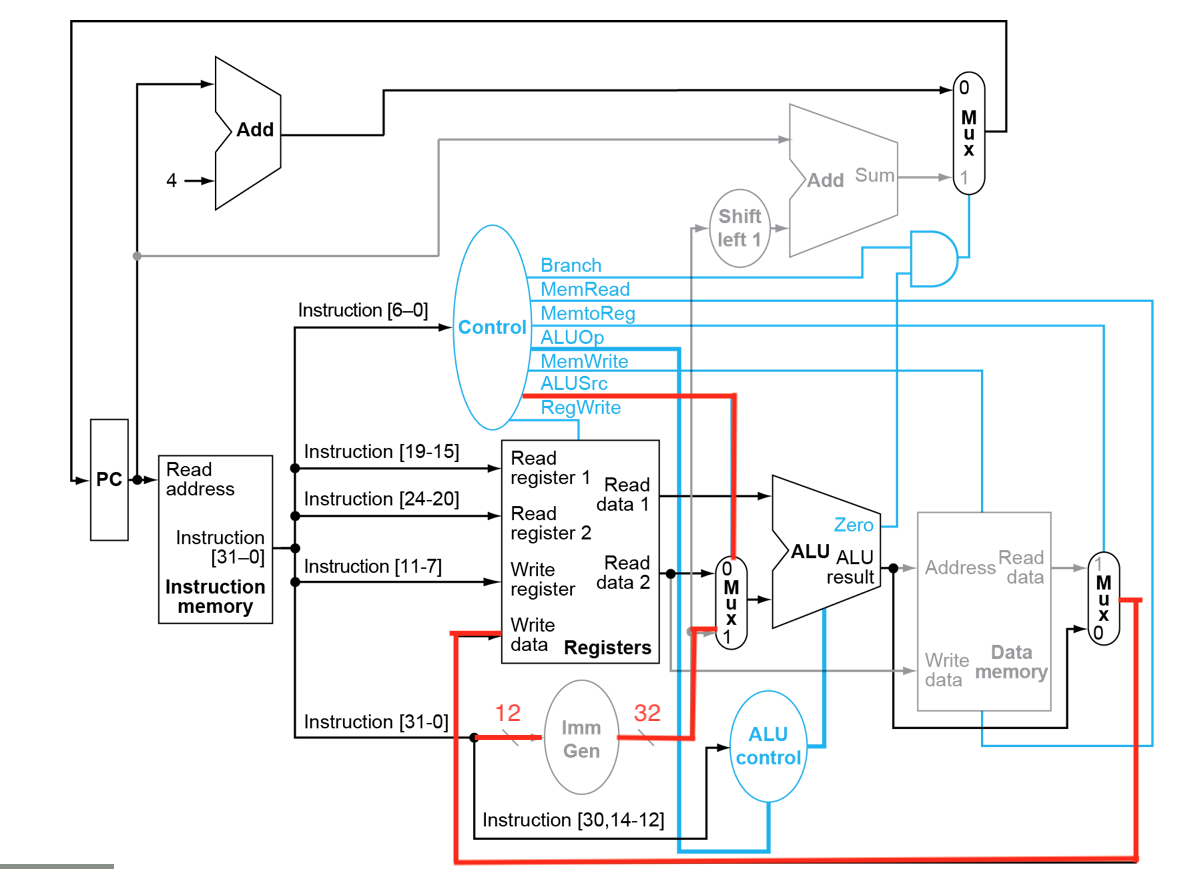
\includegraphics[width=\linewidth]{RIdatapath}
	\caption{Utype instructions datapath }
\end{figure}

\subsection{Jump( JAL, JALR) Instructions}

\begin{figure}[H]
	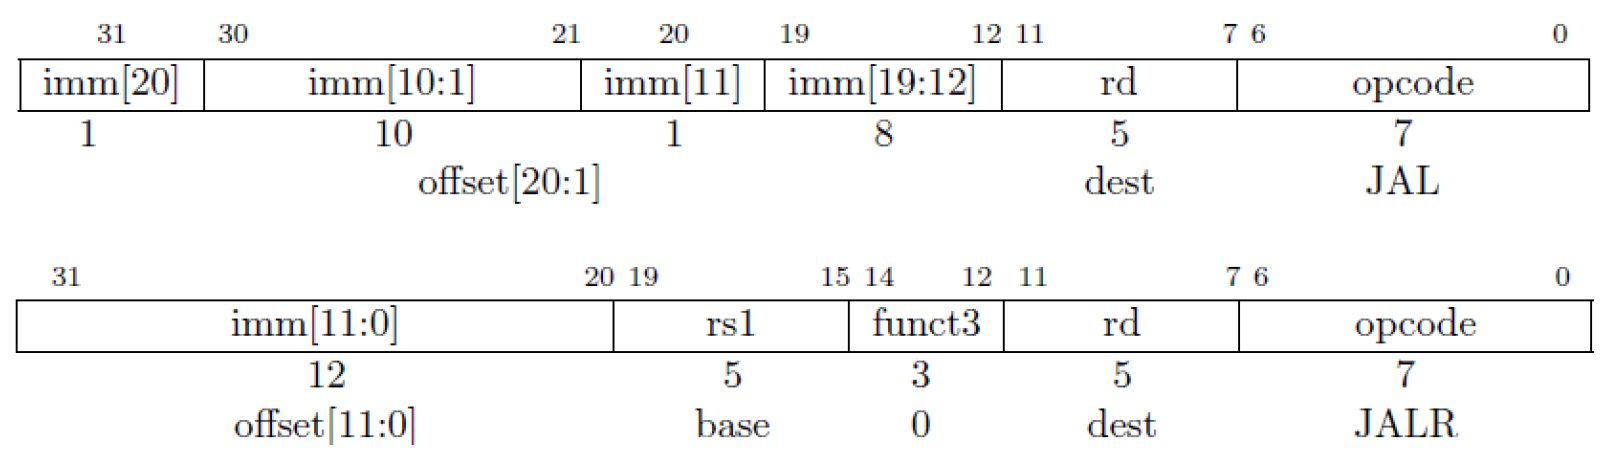
\includegraphics[width=\linewidth]{Jump}
	\caption{Snippet of Jump instructions }
\end{figure}

For JAL, the immediate gen module will sign extend the immediate value. Then, the immediate value is added to PC to get a new PC address. The PC will jump,based on the jump signal,  to that address and will execute the instruction at that taget address. Meanwhile, for jump instruction, the ALU result will be the target address plus 4, which will be stored into the destination register. 

For JALR, the immediate gen module will sign extend the immediate value. Then, the immediate value is added to Register one operand to get a new PC address. The PC will jump,based on the jump signal,  to that taget address and will execute the instruction at that taget address. Meanwhile, for jump instruction, the ALU result will be the target address plus 4, which will be stored into the destination register. 

\begin{figure}[H]
	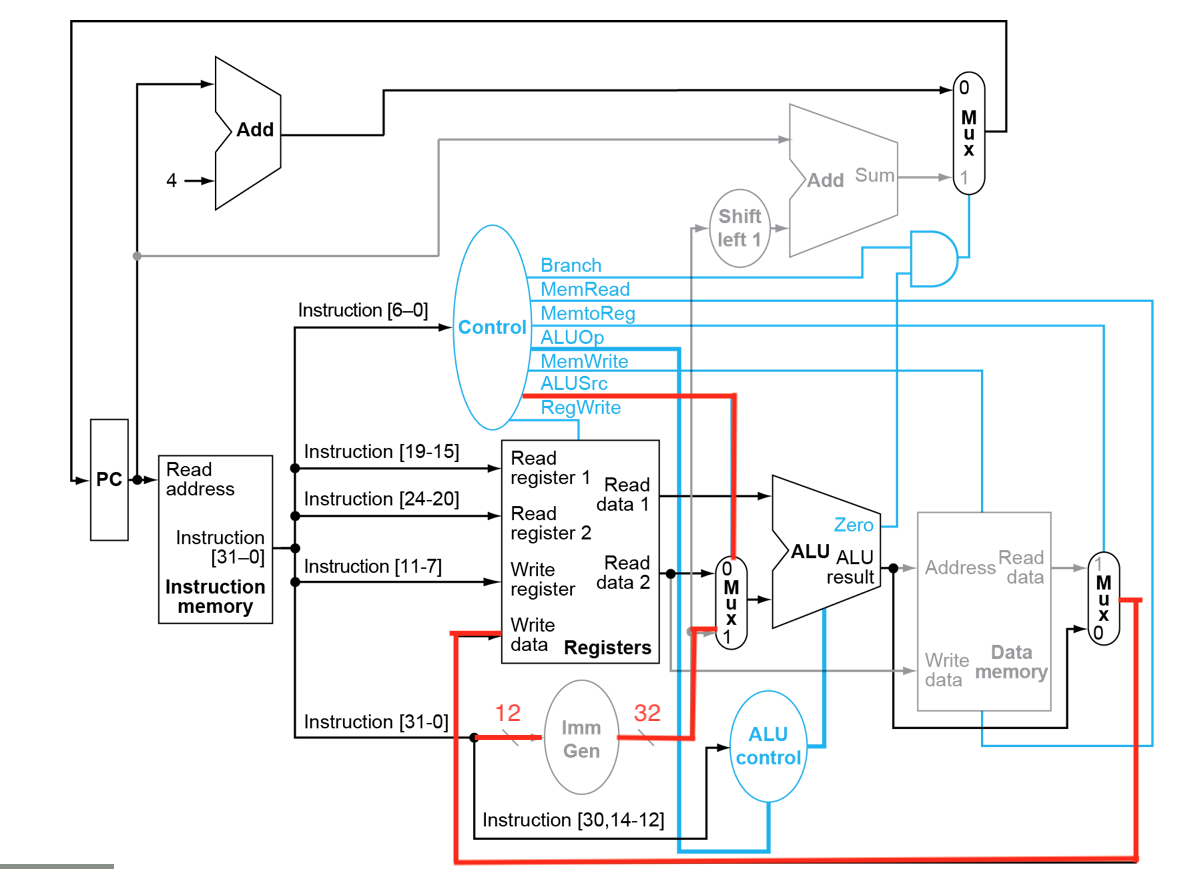
\includegraphics[width=0.9\linewidth,height=7cm]{RIdatapath}
	\caption{Jump instructions datapath }
\end{figure}


\section{Simulation Waveforms}
Here are the snippets simulation waveforms that include Clk, reset, and ALU-Result:
The simulations ran without any warnings or errors.

\begin{figure}[H]
\includegraphics[width=\linewidth]{simulation1}
\linebreak
\includegraphics[width=\linewidth]{simulation2}
\caption{Simulation snippet}
\end{figure}

\newpage
\section{Synthesis Results}
\paragraph{Report: }
The synthesis completed without any issues. Here is the synthesis report for the design implementation. 
\subsection{Timing:}

\begin{figure}[H]
	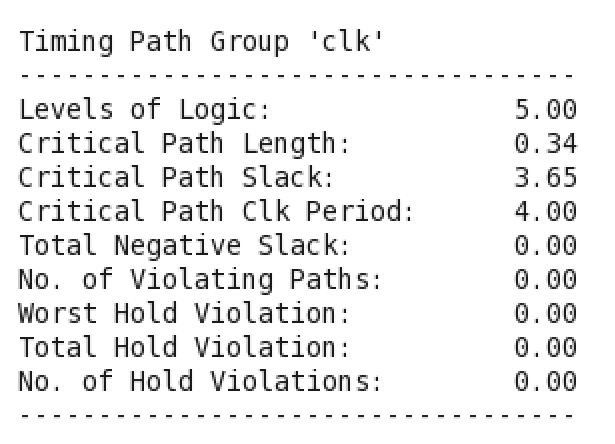
\includegraphics[width=0.9\linewidth]{Timing}
	\caption{Timing analysis }
\end{figure}

\subsection{Cell Count:}

\begin{figure}[H]
	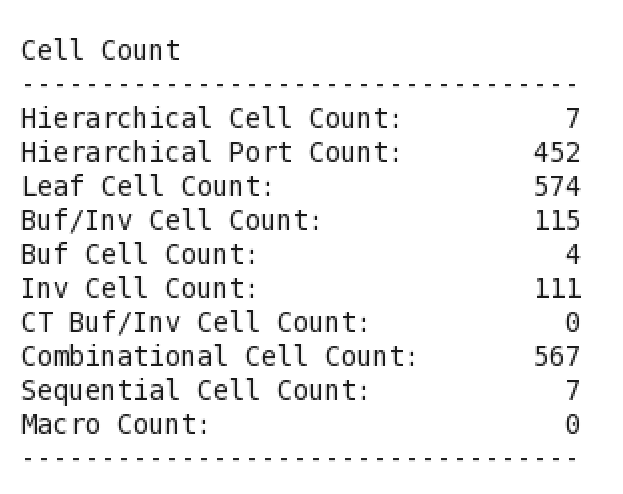
\includegraphics[width=0.9\linewidth,height=7cm]{CellCount}
	\caption{Cell count analysis }
\end{figure}

\subsection{Execution time:}

\begin{figure}[H]
	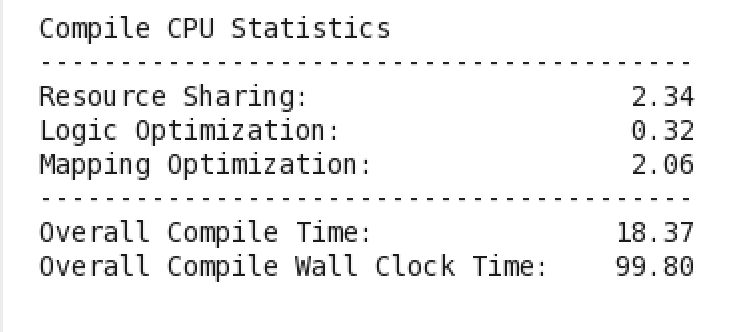
\includegraphics[width=0.9\linewidth,height=7cm]{Compiletime}
	\caption{Execution time analysis }
\end{figure}

\subsection{Area:}

\begin{figure}[H]
	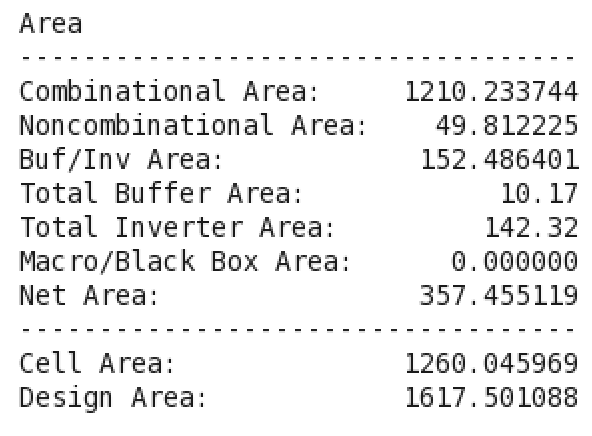
\includegraphics[width=0.9\linewidth,height=7cm]{Area}
	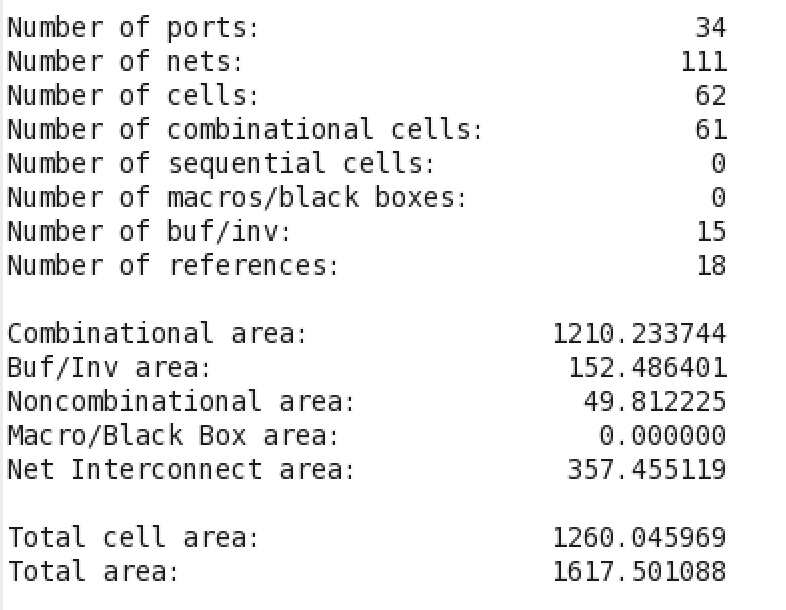
\includegraphics[width=0.9\linewidth,height=7cm]{Area2}
	\caption{Area analysis }
\end{figure}
\newpage

\subsection{Power:}

\begin{figure}[H]
	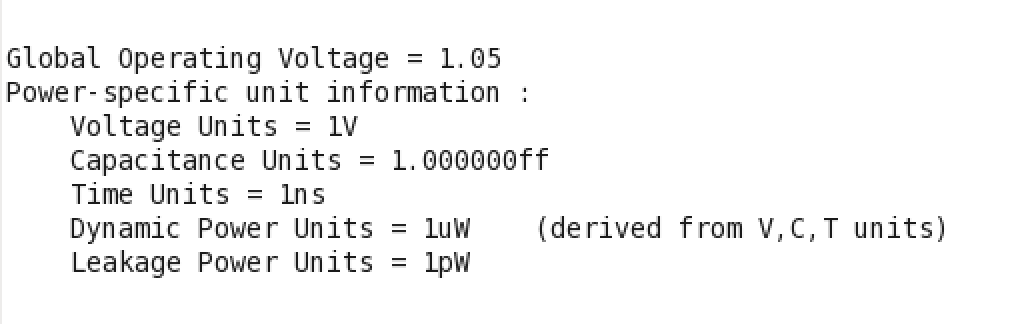
\includegraphics[width=\linewidth]{Power1}
	\linebreak
	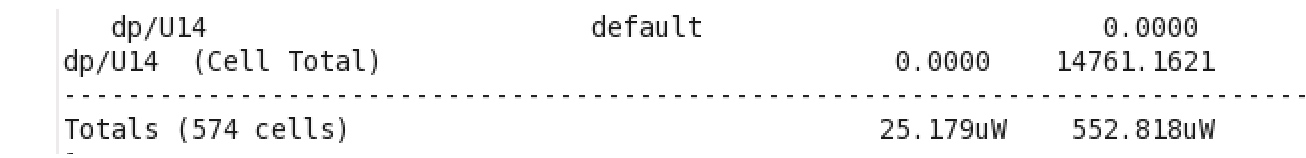
\includegraphics[width=\linewidth]{Powerf}
	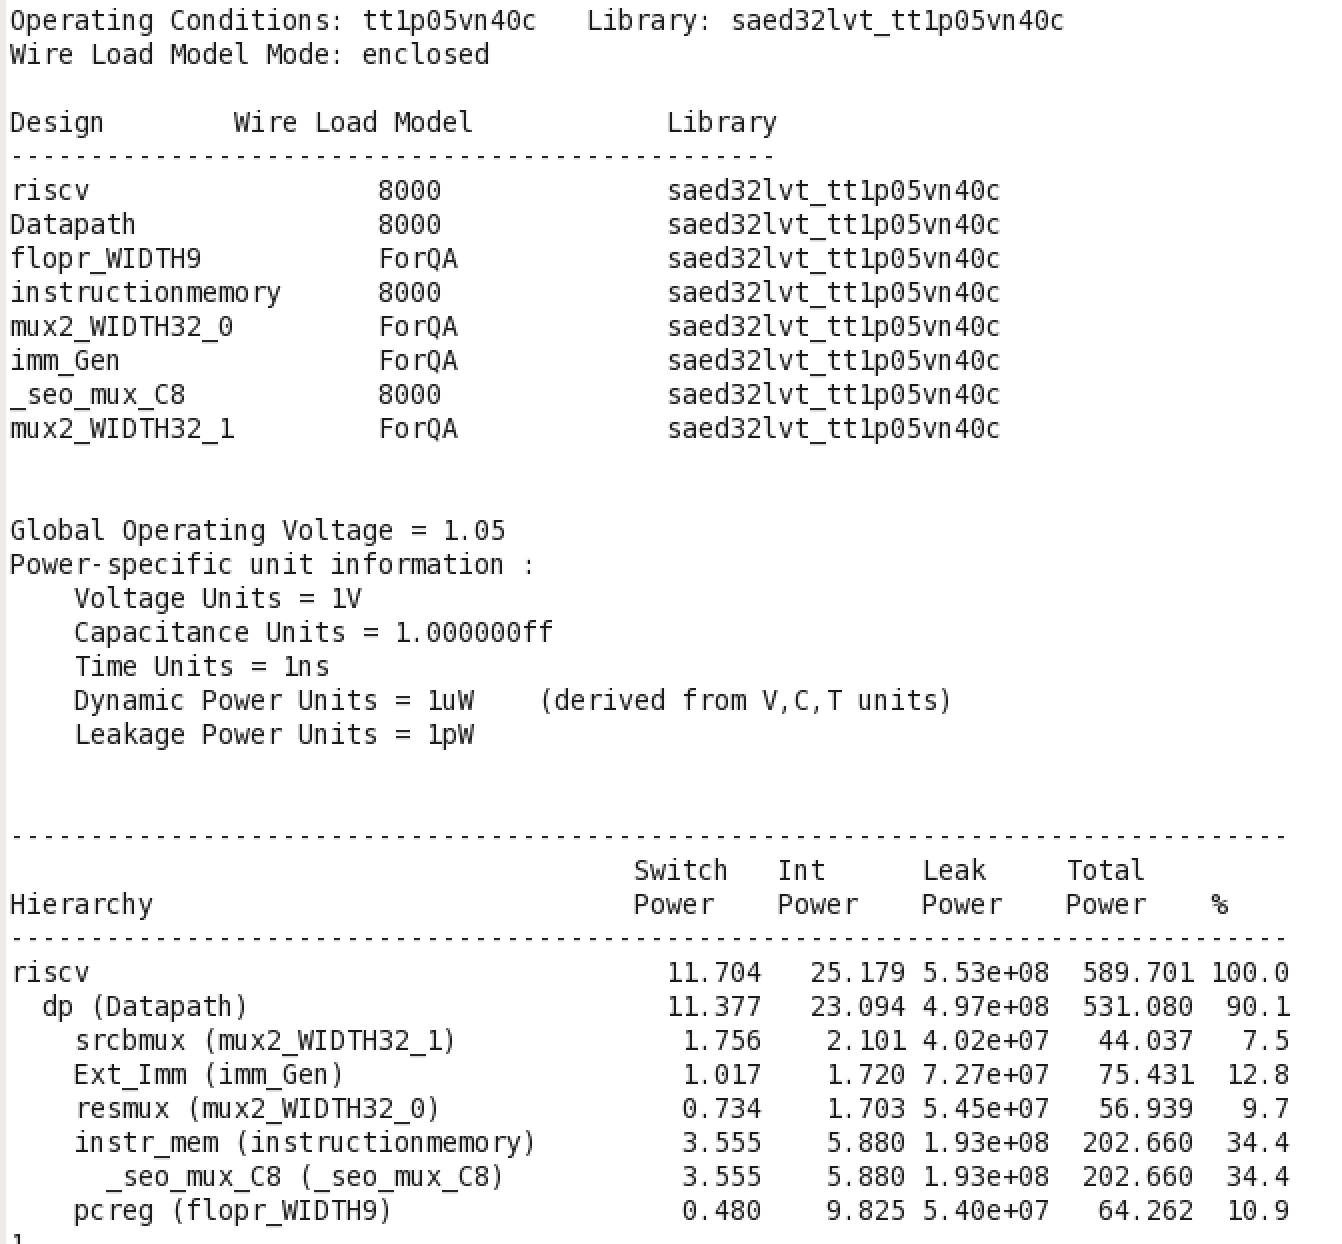
\includegraphics[width=\linewidth]{PowerHier}
	\caption{Area analysis }
\end{figure}

\subsection{Conclusion}
This Lab consisted of designing a single cycle processor. It serves well as an exposure to the real world applications. In concluding this lab, I have gained immense knowledge about the design process of processor and that will assist in future endeavors. Also, this lab sets up the groundwork for an optimized pipelined design for Lab3. 
\end{document}
